\subsection{Introduction}
\label{cic:sec:intro}

The adoption of over $21$ billion Internet of Things (IoT) devices has reshaped homes, workplaces, and industries~\cite{iotanalytics2025, memoori2025iot, mehra2020smarthome, statista_smarthome, tripathi2022role}. Vendors of smart devices---e.g., Philips Hue, Ecobee, Apple HomeKit, Siemens, Samsung SmartThings, GE Cync, Honeywell, and others~\cite{ecobee, Philips, GESync, AppleSmartThings, Honeywell, Siemens, SamsungSmartThings}---have traditionally provided their own software for users to control their devices {(through \textit{vendor-specific} interfaces), building on top of existing physical controls like buttons or switches~\cite{kodali2016iot, Khan2022Smart}}. Yet, as smart homes scale, controlling each vendor's devices separately becomes less desirable for homeowners. 

To combat the overhead of controlling each device or product individually~\cite{kaufhold2024we}, some vendors introduced {new modalities of control}, {layering additional control options on top of traditional vendor-specific interfaces}. This allows users to control both vendor-specific and cross-vendor devices through a single interface, potentially reducing overhead. For example, hubs or apps like Google Home~\cite{GoogleHome}, Apple HomeKit~\cite{apple_homekit}, or Amazon Alexa~\cite{Alexa}, enable users to control many devices (e.g., lights, thermostats, door locks) through both individual commands and automations (i.e., routines) from a single dashboard~\cite{routine-early-def, routine1, routine2}. Using such a hub, a smart home user can leverage proxy-based control to create a ``good-night'' routine that turns off their porch lights and locks their door with a voice command, even when these devices come from different vendors, without operating each device individually~\cite{sikder2022s}.

Previous research has established that vendor-specific and cross-vendor control are on opposite sides of a smart device control spectrum~\cite{10.1145/3544548.3580842,zimmermann2007universal}. {However, these control schemes may refer to \textit{how} users issue commands~\cite{geeng2019s, nichols2003studying}, \textit{which} apps or ecosystems they use~\cite{alaa2017review}, or \textit{where} the configuration logic resides (per-device rules or shared routines)~\cite{corno2021users}. In this chapter, we focus on the \textit{locus of execution} of control logic, namely whether device configuration is initiated directly on the device, or through proxies. Rather than treating one side of the spectrum as vendor-specific and the other as cross-vendor, we observe that these points are parts of an extended spectrum from \textbf{physical control}, i.e., interacting with the target device's physical controls, to \textit{varying levels} of \textbf{proxy-based control}, where user commands are routed through one or more intermediaries, such as hub apps, voice assistants, cloud services, etc., before reaching the target device~\cite{perumal2015iot, zimmermann2007universal}. For example, centralized control is one form of proxy-based control: a single proxy (or a tightly coupled set of proxies) orchestrates many devices and brands from a unified configuration layer~\cite{salman2015architecture}.}

\begin{figure}[t]
    \centering
    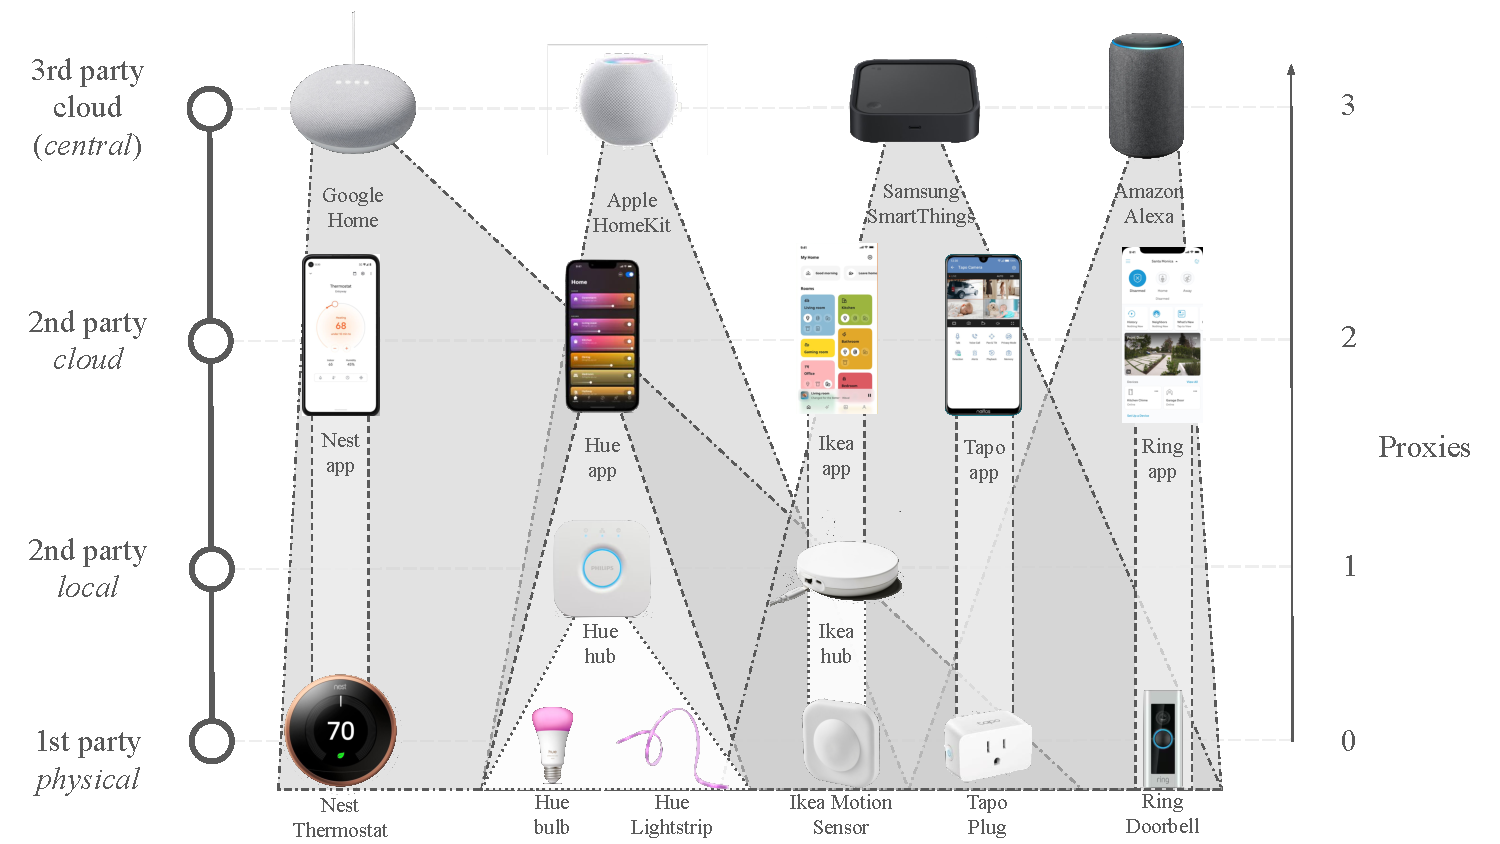
\includegraphics[width=1\linewidth,alt={Diagram of the proxy-based control spectrum, organized by locus of execution (horizontal) and proxy depth (vertical, 0 to 3 intermediary layers between user and device). At depth 0 are first-party physical devices such as the Nest thermostat, Hue bulb, and Ring doorbell; these connect upward through second-party local hubs and apps (depth 1), vendor cloud apps (depth 2), to third-party central cloud platforms such as Google Home, Apple HomeKit, Samsung SmartThings, and Amazon Alexa (depth 3). Dotted lines trace each device's control path, showing increasing indirection and centralization as the number of proxies grows.}]{ControlInContext/figures/Proxy-based Control Spectrum.pdf}
    \caption{\bf \small Proxy-based Control Spectrum. {\it Control schemes vary along two related axes. (1) Locus of execution: controls may be first-party/\textit{physical} (direct, on-device), second-party/\textit{local} (vendor hubs or LAN apps), second-party/\textit{cloud} (vendor-operated cloud services), or third-party/\textit{central} cloud ecosystems (cross-vendor platforms such as Google Home or Apple HomeKit). (2) Proxy depth: shown vertically, this indicates how many intermediary layers--hubs, vendor clouds, or central platforms--sit between the user and the device in the control path. Each control scheme has a different reach; the higher the number of proxies, the higher the degree of control centralization (breadth).}}
    
    

    \label{cic:fig:proxy-based-control-spectrum}
\end{figure}

This control spectrum (\Cref{cic:fig:proxy-based-control-spectrum}), with physical control to proxy-based\footnote{Our use of this term in this chapter is inspired by literature in the systems and networking space, which establishes the use of the ``OSI Model'' as an abstraction that encapsulates seven layers ranging from physical to application~\cite{day1983osi}.} central control as the two ends, is widely used in practice, as many homeowners rely on intermediate points on this spectrum rather than its endpoints.
Smart home device vendors offer control interfaces that can access either a single device, multiple devices from the same brand, or devices across various brands. 
{People routinely blend proxy-based and physical device control, moving across the locus of execution spectrum based on convenience, reliability, and their understanding of how the system works. These movements become especially visible during troubleshooting. 
When routines misfire, devices fail, or connectivity is unstable, users abandon usual cross-vendor proxies, fall back to device-local physical interfaces, or switch among apps and platforms~\cite{duque2022troubleshooting, alam2012review}. Troubleshooting exposes users' understandings of the smart home infrastructure, including how they choose to reveal or hide connections between devices, apps, and services. These user actions are often referred as \textit{seam practices}~\cite{kuznetsov2012seams}. Triage of device errors is a core part of living with smart homes and strongly shapes trust, preferences, and long-term configuration strategies~\cite{teigen2024troubleshooting}.}

Despite the known existence of this control spectrum,  much of the research on building operating systems (OSs) for smart homes still {\it assumes} proxy-based control is the primary way for users to interact with and control their home~\cite{HomeOS,Safehome,Transactuations}. This assumption of ``always proxy-based control'' echos how smart home OSs have traditionally been designed for machines~\cite{wulf1974hydra,golub1990mach,ritchie1974unix,unix,linux,freebsd,macos},
datacenters~\cite{tirmazi2020borg, verma2015large, schwarzkopf2013omega}, and networks~\cite{hernandezwireless, lara2013network}, domains where end-users rarely interact directly with individual devices. Empirical studies supported this disconnect by highlighting users experiencing difficulties when managing multiple dashboards for the same task~\cite{kaufhold2024we}.
In occupied homes, however, different loci of execution offer distinct capabilities and trade-offs for users, making the ``always proxy-based control'' approach incomplete. {In addition, much prior smart home control research focused on specific devices or interaction styles instead of empirical user studies~\cite{tap2016ifttt, gabhane2017smart, brackenbury2019users, wozniak2023inhabiting}.

User studies are critical for designing usable and technologically sound systems, complementing prior work that focused mainly on system proposals~\cite{oconnor2019homesnitch, DepSys, Safehome, acar2020peek}.
Moreover, existing research often abstracts away the messiness of real-world use, where devices are added gradually, apps and platforms overlap, cloud services change, and users inherit configurations set up by others. As a result, we know far less about how existing systems actually behaved in occupied homes and how people patch around misalignments across different control schemes.} 

This chapter seeks to rectify this mismatch by understanding: \textit{How do users make decisions of which control mode(s) to use across different scenarios?}
We investigate real-world workflows for interacting with smart home devices with and without proxies, giving particular attention to troubleshooting and recovery. 
We conducted a survey and follow-up interviews to understand how people combine direct device control and proxy-based control (including centralized hubs), and how breakdowns and uncertainties shape these choices. 
First, we examine how people navigate and combine different control schemes in everyday use: when and why they prefer proxy-based hubs, per-brand apps, or device-local control in different contexts. 
Second, we focus on troubleshooting as a critical moment within that broader experience. 
During troubleshooting, users' understandings of the system surface more clearly and they often reconsider which control loci they trust and are willing to invest in.

By investigating real-world workflows for interacting with smart home devices, we answer the following research questions:

\begin{itemize}
    \item \textbf{RQ1: } {\it How do smart home users navigate and combine different control schemes in their homes? } 
\end{itemize}
\begin{itemize}
    \item \textbf{RQ1a: }  {\it What factors drive users to move between, and combine, control methods within their homes?}
\end{itemize}
We also examine how device and interface breakdowns
or errors affect the above choices:
\begin{itemize}
    \item \textbf{RQ2: } {\it When smart home interactions do not go as expected, how do user perceptions of control schemes shape their responses?}
\end{itemize}
Sub-questions arise about how these experiences affect perceptions: 
\begin{itemize}
        \item \textbf{RQ2a: } {\it How do troubleshooting experiences affect users' perceptions and trust of/in their preferred smart home control methods?}
        \item \textbf{RQ2b: } {\it How does user uncertainty around functionality affect their strategies for engaging with different control methods and their seam practices?}
\end{itemize}

In summary, this chapter makes the following contributions:
\begin{itemize}
    \item We evaluate how smart home control affects a user's ability to meet their smart home goals, and find that \textbf{\textit{the spectrum of smart device control plays a major role}} in user preferences and experiences in managing and using their smart home devices.
    \item We reveal how and why users decide to control their devices at different points along the proxy-based to direct device control spectrum, exposing the different seams within their smart homes, understanding that  \textbf{\textit{users move freely along the spectrum, guided by situational factors such as convenience, task, and perceived reliability}}.
    {
    \item We characterize troubleshooting workflows and seam practices across control schemes, and detail how breakdowns and uncertainties prompt users to \textit{\textbf{reconfigure control arrangements, fall back to direct device control, and strategically reveal or hide infrastructural seams when troubleshooting.}}
    }
    \item We identify and understand the factors that guide smart home control preferences and suggest ways for future research and design to incorporate these perspectives, namely \textbf{\textit{accounting for spatial and temporal heterogeneity}} in smart homes, as well as \textbf{\textit{supporting movement through varying seam hiding/revealing practices along the smart home control spectrum}}.
\end{itemize}

